\documentclass[12pt,a4paper]{article}
\usepackage[utf8]{inputenc}
\usepackage[spanish]{babel}

% Paquetes

\usepackage{amsmath}
\usepackage{amsfonts}
\usepackage{amssymb}
\usepackage{amsthm}  % Permite crear teoremas nuevos / Estilos de teoremas 
\usepackage{graphicx} % 
\usepackage[colorlinks=true,allcolors=blue]{hyperref} % Crea las hiperreferencias (clicas y te mueves)
\graphicspath{{Figuras/}}
\usepackage{fancybox} % para usar la caja de los ejemplos

% Autor y titulo

\title{Práctica Fran-Hertz Mercurio}
\author{Daniel Vázquez Lago}

% Forma del  texto

\setlength{\parindent}{15px}
\usepackage[left=2.25cm,right=2cm,top=4cm,bottom=2cm]{geometry}

% Otros


\numberwithin{equation}{section}
\numberwithin{figure}{section}

% Comandos propios
\newcommand{\tquad}{\quad \quad \quad}

\newcommand{\parentesis}[1]{\left( #1  \right)}
\newcommand{\parciales}[2]{\frac{\partial #1}{\partial #2}}
\newcommand{\pparciales}[2]{\parentesis{\parciales{#1}{#2}}}
\newcommand{\ccorchetes}[1]{\left[ #1  \right]}
\newcommand{\D}{\mathrm{d}}
\newcommand{\derivadas}[2]{\frac{\D #1}{\D #2}}
\newcommand{\cte}{\mathrm{cte}}

\newcommand{\Tr}{\mathrm{Tr} \ }


\newcommand{\eup}{\mid \uparrow \rangle}
\newcommand{\edw}{\mid \downarrow \rangle}

\newcommand{\Hcal}{\mathcal{H}}
% Comandos vectoriales

\newcommand{\xn}{\mathbf{x}}
\newcommand{\yn}{\mathbf{y}}
\newcommand{\zn}{\mathbf{z}}
\newcommand{\vn}{\mathbf{v}}
\newcommand{\un}{\mathbf{u}}
\newcommand{\rn}{\mathbf{r}}
\newcommand{\qn}{\mathbf{q}}
\newcommand{\pn}{\mathbf{p}}
\newcommand{\kn}{\mathbf{k}}
\newcommand{\sn}{\mathbf{s}}
\newcommand{\an}{\mathbf{a}}
\newcommand{\bn}{\mathbf{b}}
\newcommand{\nn}{\mathbf{n}}

\newcommand{\rhon}{\mathbf{\rho}}


\newcommand{\An}{\mathbf{A}}
\newcommand{\Pn}{\mathbf{P}}
\newcommand{\Bn}{\mathbf{B}}
\newcommand{\Sn}{\mathbf{S}}
\newcommand{\En}{\mathbf{E}}
\newcommand{\Hn}{\mathbf{H}}
\newcommand{\Encal}{\boldsymbol{\mathcal{E}}}
\newcommand{\mun}{\boldsymbol{\mu}}


% Comandos vectoriales unitarios

\newcommand{\hrho}{\hat{\rhon}}
\newcommand{\hnu}{\hat{\un}}
\newcommand{\hns}{\hat{\sn}}
\newcommand{\hnr}{\hat{\rn}}
\newcommand{\hnx}{\hat{\xn}}
\newcommand{\hny}{\hat{\yn}}
\newcommand{\hnz}{\hat{\zn}}

% Comandos teoremas

\newtheorem{theorem}{Teorema}[section]
%\theoremstyle{definition}
\newtheorem{definition}{Definicion}[section]

\begin{document}

\maketitle

\newpage

\tableofcontents

\newpage

\section{Objetivos}

El principal objetivo de esta práctica es calcular el valor de la energía de excitación del mercurio, que llamaremos $\Delta E$.

\section{Introducción teórica}

Como hemos dicho queremos calcular el nivel de excitación del mercurio, es decir, la energía necesaria para que un electrón pase de su primer orbital al primer orbital excitado. Para evaluar dicha energía James Frank y Gustav Hertz diseñaron un experimento muy interesante, que es el que usaremos aquí. \\

El experimento consiste, de manera muy resumida, en emitir electrones desde un ánodo, y recibirlos en un cátodo en el otro extremo del tubo. La energía que tengan los electrones la podremos controlar nosotros en el laboratorio. Mientras la energía no sea muy grande, la corriente entre ánodo y cátodo no se verá alterada, dado que el choque electrón-átomo es un choque inelástico. Sin embargo cuando el electrón consiga determinada energía (la energía de excitación del mercurio) el choque con los átomos de mercurio transferirá toda la energía cinética del electrón para excitar el átomo de mercurio, convirtiéndose en una colisión inelástica. Esto hará que el número de electrones que llega al cátodo descienda, haciendo que veamos un pico en la intensidad. \\

Si siguieramos aumentando la energía de los electrones, aún tras el primer choque conservará suficiente energía cinética para llegar al cátodo, restableciendo la intensidad. De nuevo, cuando la energía cinética del electrón sea suficiente como para excitar átomos de manera consecutiva, la corriente volverá a descender. Así obtendremos una serie de máximos y mínimos de intensidad que nos permitirá calcular la energía cinética de los electrones. \\

Debido a la construcción del experimento, la energía a partir la cual vemos el primer mínimo no será la energía de excitación. Esto se debe principalmente a que existen factores (que podemos llamar $V_{off}$) que hacen que el voltaje a partir el cual se ve el primer mínimo venga dado por:

\begin{equation}
U_{\min}^{1}  = U + V_{off}
\end{equation}
A partir de este voltaje no podremos calcular el voltaje de exitación ($U$), i.e. el voltaje que hay que aplicar a un electrón para que en el choque con un átomo de mercurio y se excita ($\Delta E = e \cdot U$). Sin embargo si consideramos la energía a partir la cual aparece el segundo mínimo:

\begin{equation}
U_{\min}^{2} = 2U + V_{off}
\end{equation}
podemos ver claramente como la diferencia de $U_{\min}^{2}$ y $U_{\min}^{1}$ si nos permitiría eliminar esta energía de offset. De esta manera podremos obtener la energía de excitación a partir de las diferencias de voltaje entre mínimos consecutivos, ya que:

\begin{equation}
U = U_{\min}^{n+1} - U_{\min}^{n} 
\end{equation}
donde $U_{\min}^{n}$ simboliza el potencial del mínimo número $n$. Una vez hemos entendido como extraer el nivel de energía a partir de la exitación del mercurio solo queda analizar los datos experimentales, encontrar los mínimos y asignarles una incertidumbre. Una pregunta que desde ya nos podemos plantear es: ¿La diferencia entre máximos, dado que se encuentran a mitad de camino entre un mínimo y otro, no servirían también para calcular $U$? Como el proceso usado para obtener los mínimos es el mismo  que nos permite calcular los máximos, sin más esfuerzo que redactar un poco más, podremos ver si los resultados usando los máximos son iguales o parecidos que usando los mínimos, o si por el contrario son diferentes. De ser diferentes tendremos que buscar una razón. \\

Debemos mencionar que cada toma de datos se realizado para un potencial de retardo diferente y constante en cada medida. El potencial de retardo $U_2$ ; ahora diferenciamos de $U_1$, el potencial que metemos a los electrones; es básicamente un potencial que reduce la velocidad de los electrones a medida que van cruzando el tubo. De esta manera el potencial de retardo no permite llegar al cátodo a aquellos electrones con una baja energía cinética. Por esa misma razón a medida que aumentemos $U_2$ los picos de los máximos serán  menores. Eso se puede ver perfectamente en la figura $\ref{Fig:1.0}$. 

 
\section{Análisis de los resultados}

En esta parte vamos a calcular los mínimos y máximos usando dos métodos. El primero de ellos es un método computacional que el propio programa que usamos para obtener los datos, nos asigna. Estos no vienen con incertidumbre, por tanto deberemos nostros a mano asignarle unos. El otro método consiste en aproximar la región del mínimo/máximo para calcular una parábola. A partir de los coeficientes de la parábola calcularemos $U_n$. Entonces en esta sección vamos a analizar como se obtienen los mínimos/máximos, y comentar las incertidumbres de cada valor. Tras esto calcularemos las energías a partir de los mínimos, obteniendo así una cantidad de 8 energías para cada $U_2$ usada (4 energías por haber 5 mínimos, y otras 4 por haber 5 máximos). 

\subsection{Obtención usando el programa del laboratorio}

Como hemos mencionado el programa del laboratorio ya nos da, aproximadamente, un valor para los máximos y otros para los mínimos. Sin embargo el valor que nos da es un valor sin incertidumbres, por lo que habrá que asignarle una de manera completamente arbitraria. Nosotros hemos elegido $\sigma = 0.25$ ya que nos parece el rango donde con una seguridad del 95\% el valor del máximo/mínimo cae. Los datos calculados así se presentan en las tablas del apartado \ref{Subsubsec:6.1.2}, y en las gráficas \ref{Fig:3.11}, \ref{Fig:3.21}, \ref{Fig:3.31}, \ref{Fig:3.41} , \ref{Fig:3.51} y \ref{Fig:3.61}.


\subsection{Obtención usando la aproximación parabólica}

Como sabemos una parábola viene determinada por la función $f(x)=a+bx+cx^2$. Para calcular la posición donde se encuentra su punto mínimo (o máximo) solo debemos derivar e igualar a cero. En ese caso podemos obtener que el mínimo/máximo se encuentra en la posición:

\begin{equation}
x_0 = -\frac{b}{2c}
\end{equation}
por lo que la incertidumbre de cada máximo/mínimo viene determinada por la fórmula:

\begin{equation}
s(x_0) = \sqrt{\parentesis{\frac{s(b)}{2c}}^2 + \parentesis{\frac{s(c)\cdot b}{2c^2}}^2}
\end{equation}
La incertidumbre será mayor o menor en función de la cantidad de datos y la dispersión de estos, por lo que consideramos que no hay ningún motivo para añadir una incertidumbre mayor que esta, dada por los coeficientes de las regresiones parabólicas. Los datos calculados se encuentran en las tablas del apartado \ref{Subsubsec:6.1.1}, y en las gráficas \ref{Fig:2.1}, \ref{Fig:2.2}, \ref{Fig:2.3}, \ref{Fig:2.4}, \ref{Fig:2.5} y \ref{Fig:2.6}.

\subsection{Dependencia de $U_2$}

Como podemos ver en las tablas (para cualquier método de obtención) los máximos y mínimos se desplazan en función de los valores de $U_2$. A priorí esto  no debería de importarnos, ya que nos importa la diferencias entre los mínimos/máximos. De hecho, esta dependencia no acaba afectando a las diferencias entre los extremos, y por tanto $\Delta E = e \cdot U$ no se ve afectada. 

\subsection{Cálculo de la energía}

Una vez hemos obtenido los valores de los mínimos podemos calcular la energía. Podemos hacerlo de varias formas, podemos calcular la diferencia entre el mínimo más grande y el mínimo más grande (análogamente los máximos) y dividir entre 4. Dado que tenemos todos los mínimos y máximos que menos que calcular la diferencia entre cada uno de estos. Esto mismo hemos hecho en las tablas de los apartados \ref{Subsubsec:6.1.3} y \ref{Subsubsec:6.1.4} donde $n-m$ significa que es la diferencia de energía dada entre el mínimo/máximo número $n$ y número $m$. \\

La incertidumbre de cada valor de la energía viene dada por la inceritdumbre del mínimo $n$ y $m$, esto es:

\begin{equation}
s(\Delta E) = e \cdot \sqrt{s(U_{n})^2+s(U_{m})^2}
\end{equation}
Por esta misma razón la incertidumbre de los valores de los laboratorios (apartado \ref{Subsubsec:6.1.4}) es la misma para todos, ya que $s(U_n)=s(U_m)$. Otra cualidad de los datos es que varía bastante en función de las posiciones $n-m$, en general siendo $\Delta E$ mas grande cuanto mas grande es $n-m$, lo cual será foco de debate en la siguiente sección.

\section{Conclusiones}

En este apartado calcularemos los valores medios de las energías, comparándolos con los valores teóricos; discutiremos las razones por las que $\Delta E$ cambia en función de $n-m$ (presentando una tabla); y por qué $\Delta E_{\max}$ da un diferente resultado que $\Delta E_{\min}$ en las tablas  \ref{Tab:Em-1-par} y \ref{Tab:Em-2-lab}.  \\

\subsection{Diferencias entre máximos y mínimos}


Como podemos ver en las tablas \ref{Tab:Em-1-par} y \ref{Tab:Em-2-lab}, los datos de los máximos son sobre 0.10-0.15 eV diferentes. Sin embargo nosotros hemos dicho en la teoría que deberían ser parecidos a los valores de $\Delta E_{\min}$. ¿Como es esto posible? Para esto debemos fijarnos en las tablas de los apartados \ref{Subsubsec:6.1.3} y  \ref{Subsubsec:6.1.4}. Como podemos ver en los $\Delta E_{\max}^{2-3}, \Delta E_{\max}^{3-4}$ y $\Delta E_{\max}^{4-5}$ son parecidos (aproximadamente con 0.01 eV menores), siendo la diferencia $\Delta E_{\max}^{1-2}$ la que realmente es diferente respecto $\Delta E_{\min}^{1-2}$ (unos 0.5 eV). Es decir, es el primer máximo el que esta alterando en gran medida $\Delta E_{\max}$ para ambos métodos. La existencia de un potencial de retardo hace que el primer máximo no caiga necesariamente en $U_{\max}^1=U_{\min}^1/2$, alterando en gran medida el valor. Si realizamos el valor medio pero ahora sin usar los valores de los primeros máximos podemos ver que sí se parecen \ref{Tab:Em-1-sin-par} y \ref{Tab:Em-2-sin-lab}. Sin este valor podemos observar que experimentalmente dan prácticamente el mismo resultado, por lo que usar los máximos es, al menos para nuestros datos, tan válido como usar los mínimos.


\subsection{Dependencias de $\Delta E$}

En esta sección vamos a estudiar si $\Delta E$ depende de $U_1$ y $U_2$. En otras palabras: vamos a ver si $\Delta E$ crece/decrece en función de $U_1$, y si crece/decrece al aumentar $U_2$. \\

Llamaremos a $n$ el ``orden del extremo'', de tal manera que tendremos 1 para los extremos 1-2, 2 para los extremos 2-3... Como podemos ver en las tablas del apartado \ref{Subsubsec:6.1.3} y las figuras \ref{Fig:6.2.2.1} y \ref{Fig:6.2.2.2} (en las cuales hemos representado $\Delta E$ en función de n), tenemos que $\Delta E_{min}$ y $\Delta E_{max}$ aumenta cuando $n$ aumenta, esto es, que aumenta cuando $U_1$ aumenta. ¿A qué se debe esto?  Una de la razones podría ser que, con un potencial tan grande, no se excite del estado fundamental al primer estado, si no que se exciten otros. Un estudio de las ondas de luz emitidas por el mercurio nos podría solventar esta duda. Otras razones pueden ser algún tipo de interacción del mercurio con el cátodo o ánodo, entre otras. Habría que hacer un estudio mas profundo de la teoría y de las colisiones atómicas, algo fuera de nuestro alcance. En las tablas del apartado \ref{Subsubsec:6.1.4} (figura \ref{Fig:6.2.2.4}). ocurre un fenómeno similar a la del apartado anterior, aunque de una manera menos pronunciada, ya que tiene un comportamiento más irregular respecto $U_1$. Sin embargo para este método podemos ver que este patrón es mucho mas irregular, tal y como podemos ver en la figura \ref{Fig:6.2.2.3}. \\

El valor de $\Delta E$ no varía al cambiar $U_2$ (si que varía, al ser experimentos diferentes, pero la variación no muestra signos de un patrón claro), ni en un método ni en otro (tal y como hemos comentado anteriormente). De hecho esto se puede ver en las tablas \ref{Tab:Em-1-sin-par} y \ref{Tab:Em-2-sin-lab}, ya que los valores medios no prácticamente no varían según $U_2$. Lo único que ocurre al variar $U_2$ es que el valor de las incertidumbres aumenta (lo cual es normal, ya que las aproximaciones son peores). 

\subsection{Energía de excitación del mercurio: teórico vs experimental}

Para comparar el valor medio de los los $\Delta E$ para mínimos y máximos (la última fila de las tablas \ref{Tab:Em-1-sin-par} y \ref{Tab:Em-2-sin-lab}) con el dato teórico primero tendremos que dar un valor al dato teórico. En el guión se nos dice que el valor real es: \\

\begin{equation}
\Delta E^{teo} = 4.886 \ (\mathrm{eV})
\end{equation}
Para que se pueda comparar rápidamente de un vistazo, sin tener que ira las tablas, escribimos el valor medio experimental para cada método: 


\begin{equation}
\Delta E_{\max}^{par} = 4.804 \ (\mathrm{eV}) \quad \quad   s\parentesis{\Delta E_{\max}^{par}}= 0.095 \ (\mathrm{eV})
\end{equation} 

\begin{equation}
\Delta E_{\max}^{par} =  4.826  \ (\mathrm{eV}) \quad \quad s\parentesis{\Delta E_{\max}^{par}}=  0.089 \ (\mathrm{eV}) 
\end{equation}

\begin{equation}
\Delta E_{\max}^{lab} = 4.802 \ (\mathrm{eV}) \quad \quad  s\parentesis{\Delta E_{\max}^{lab}}= 0.067 \ (\mathrm{eV}) 
\end{equation} 

\begin{equation} 
\Delta E_{\max}^{lab} =  4.843  \ (\mathrm{eV}) \quad \quad  s\parentesis{\Delta E_{\max}^{lab}}=  0.058 \ (\mathrm{eV}) 
\end{equation}

Dado que los  resultados finales son pocos, realizar un test estadístico para hallar la relación no va a resultar nada complejo ni engorroso. El test usado va a ser un test de Student, esto es, el  test típico de la media de una población normal. Dado que esto es una memoria y no un manual de tratamiento de datos o estadística, simplemente diremos que con un grado de confianza $1-\alpha$ ($\alpha$  representa la probabilidad de cometer un error tipo I, o lo que es lo mismo, rechazar incorrectamente la hipótesis nula) aceptamos o rechazamos la hipótesis de que $\Delta E^{teo}$ es correcta. Entonces calculamos el $t$ para cada medida ($t=(\bar{x}-x_{teo})/\sqrt{s/n}$; con n=4 al hacer la media con 4 valores). En ese caso:

\begin{equation}
t_{\min}^{lab} = 0.254 \quad
t_{\max}^{lab} = 0.459 \quad
t_{\min}^{par} = 0.283 \quad
t_{\max}^{par} = 0.375
\end{equation}
ahora tenemos que compararlo con el valor tabulado con, por ejemplo un $\alpha=0.05$. Si ocurre que $t>t_{\mathrm{tabulado}}$ tendremos que rechazar la hipótesis. Si por el contrario tenemos que $t\leq t_{\mathrm{tabulado}}$ podremos decir que $\Delta E^{teo}$ . Esto en la literatura se le llama \textit{test de hipótesis estadística}. En cualquier caso para $\alpha=4$, $n=4$ (3 grados de libertad) tenemos que $t_{\mathrm{tab}}=2.132$, ergo aceptamos el valor $\Delta E_{teo}$ a con un nivel de significación del 95\%. Véase referencia \cite{libro-1} para la tabulación usada, y en más en general, el tratamiento de datos.  \\

\subsection{Impresiones finales}

Como podemos ver hemos concluido satisfactoriamente la memoria, ya que aun que los datos no cuadren perfectamente con el valor teórico (una diferencia entorno a los 0.04-0.08 eV) el resultado es lo suficientemente conclusivo como para no rechazar el dato. Más allá de esto hemos podido comprobar no solo la verifiación de este hecho experimental, si no que además hemos visto como funciona la dependencia de $\Delta E$ respecto $U_1$ y $U_2$, así como la diferencia entre usar máximos y mínimos. Aunque hayamos ampliado considerablemente el objetivo inicial de la práctica, en lo personal me encuentro bastante satisfecho. Este último hecho nos ha permitido ver de primerea mano como los orbitales estan cuantizados, tal y como vieron Frank y Hertz, demostrando así (para sus coetáneos) que el modelo de Bohr era correcto, aunque nosotros ahora sepamos que es \textit{incompleto}. \\

Lo único que ampliaría sería el rango de $U_2$ para estudiar (así ver si realmente existe una dependencia de con $U_2$) y un mayor rango de $U_1$. También podríamos calcular $h$ a partir de esta $\Delta E$ si conociéramos la longitud de onda emitida por la primera excitación, y dado que esta prácticamente es relativamente corta de realizar, podríamos haberlo hecho perfectamente, y así hacer un poco mas completa la práctica. 


\section{Anexo}
\subsection{Tablas de datos}
\subsubsection{Extremos por aproximación parabólica} \label{Subsubsec:6.1.1}

%\hline & $U_1^{\max}$ (V) & s($U_1^{\max}$) (V) & $U_1^{\min}$ (V) & s($U_1^{\min}$) (V) \\
  
\begin{table}[h!] 	 \centering 
\begin{tabular}{ccccc}
\hline & $U_1^{\max}$ (V) & s($U_1^{\max}$) (V) & $U_1^{\min}$ (V) & s($U_1^{\min}$) (V) \\
\hline
 1 & 12.02 & 0.15 & 13.84 & 0.14 \\
 2 & 16.38 & 0.08 & 18.52 & 0.17 \\
 3 & 21.05 & 0.16 & 23.25 & 0.11 \\
 4 & 25.88 & 0.33 & 28.17 & 0.15 \\
 5 & 30.81 & 0.42 & 33.15 & 0.20 \\
\hline
\end{tabular}\caption{Extremos para $U_2=0.40$ V usando la aproximación-parabólica.} 
\label{Tab:parabolas-1} 
\end{table} 
 
 
\begin{table}[h!] 	 \centering 
\begin{tabular}{ccccc}
\hline & $U_1^{\max}$ (V) & s($U_1^{\max}$) (V) & $U_1^{\min}$ (V) & s($U_1^{\min}$) (V) \\
\hline
 1 & 12.04 & 0.22 & 13.86 & 0.23 \\
 2 & 16.42 & 0.12 & 18.56 & 0.12 \\
 3 & 21.08 & 0.13 & 23.30 & 0.21 \\
 4 & 25.93 & 0.28 & 28.22 & 0.23 \\
 5 & 30.85 & 0.29 & 33.20 & 0.28 \\
\hline
\end{tabular}\caption{Extremos para $U_2=0.50$ V usando la aproximación-parabólica.} 
\label{Tab:parabolas-2} 
\end{table} 
 
 
\begin{table}[h!] 	 \centering 
\begin{tabular}{ccccc}
\hline & $U_1^{\max}$ (V) & s($U_1^{\max}$) (V) & $U_1^{\min}$ (V) & s($U_1^{\min}$) (V) \\
\hline
 1 & 12.04 & 0.19 & 13.92 & 0.27 \\
 2 & 16.45 & 0.13 & 18.62 & 0.19 \\
 3 & 21.11 & 0.10 & 23.35 & 0.20 \\
 4 & 25.95 & 0.25 & 28.25 & 0.19 \\
 5 & 30.87 & 0.51 & 33.22 & 0.33 \\
\hline
\end{tabular}\caption{Extremos para $U_2=0.60$ V usando la aproximación-parabólica.} 
\label{Tab:parabolas-3} 
\end{table} 

\newpage 
 
\begin{table}[h!] 	 \centering 
\begin{tabular}{ccccc}
\hline & $U_1^{\max}$ (V) & s($U_1^{\max}$) (V) & $U_1^{\min}$ (V) & s($U_1^{\min}$) (V) \\
\hline
 1 & 12.16 & 0.21 & 14.05 & 0.23 \\
 2 & 16.56 & 0.12 & 18.75 & 0.18 \\
 3 & 21.23 & 0.13 & 23.49 & 0.22 \\
 4 & 26.04 & 0.19 & 28.41 & 0.22 \\
 5 & 30.97 & 0.50 & 33.39 & 0.29 \\
\hline
\end{tabular}\caption{Extremos para $U_2=1.00$ V usando la aproximación-parabólica.} 
\label{Tab:parabolas-4} 
\end{table} 
 
 
\begin{table}[h!] 	 \centering 
\begin{tabular}{ccccc}
\hline & $U_1^{\max}$ (V) & s($U_1^{\max}$) (V) & $U_1^{\min}$ (V) & s($U_1^{\min}$) (V) \\
\hline
 1 & 12.24 & 0.29 & 14.33 & 0.30 \\
 2 & 16.69 & 0.21 & 18.97 & 0.37 \\
 3 & 21.34 & 0.23 & 23.71 & 0.28 \\
 4 & 26.18 & 0.32 & 28.62 & 0.23 \\
 5 & 31.10 & 0.32 & 33.57 & 0.55 \\
\hline
\end{tabular}\caption{Extremos para $U_2=1.50$ V usando la aproximación-parabólica.} 
\label{Tab:parabolas-5} 
\end{table} 
 
 
\begin{table}[h!] 	 \centering 
\begin{tabular}{ccccc}
\hline & $U_1^{\max}$ (V) & s($U_1^{\max}$) (V) & $U_1^{\min}$ (V) & s($U_1^{\min}$) (V) \\
\hline
 1 & 12.42 & 0.40 & 14.49 & 0.41 \\
 2 & 16.85 & 0.31 & 19.14 & 0.32 \\
 3 & 21.49 & 0.39 & 23.91 & 0.45 \\
 4 & 26.32 & 0.24 & 28.81 & 0.62 \\
 5 & 31.24 & 0.64 & 33.78 & 0.87 \\
\hline
\end{tabular}\caption{Extremos para $U_2=2.00$ V usando la aproximación-parabólica.} 
\label{Tab:parabolas-6} 
\end{table} 


\subsubsection{Extremos laboratorio} \label{Subsubsec:6.1.2}
 
 \begin{table}[h!] 	 \centering 
\begin{tabular}{ccccc}
\hline & $U_1^{\max}$ (V) & s($U_1^{\max}$) (V) & $U_1^{\min}$ (V) & s($U_1^{\min}$) (V) \\
\hline
 1 & 11.99 & 0.20 & 13.87 & 0.20 \\
 2 & 16.36 & 0.20 & 18.73 & 0.20 \\
 3 & 21.09 & 0.20 & 23.32 & 0.20 \\
 4 & 25.86 & 0.20 & 28.20 & 0.20 \\
 5 & 30.76 & 0.20 & 33.11 & 0.20 \\
\hline
\end{tabular}\caption{Extremos para $U_2=0.40$ V usando datos laboratorio.} 
\label{Tab:lab-1} 
\end{table} 
\newpage
 
 
\begin{table}[h!] 	 \centering 
\begin{tabular}{ccccc}
\hline & $U_1^{\max}$ (V) & s($U_1^{\max}$) (V) & $U_1^{\min}$ (V) & s($U_1^{\min}$) (V) \\
\hline
 1 & 11.94 & 0.20 & 14.06 & 0.20 \\
 2 & 16.31 & 0.20 & 18.65 & 0.20 \\
 3 & 21.09 & 0.20 & 23.44 & 0.20 \\
 4 & 25.95 & 0.20 & 28.20 & 0.20 \\
 5 & 30.81 & 0.20 & 33.18 & 0.20 \\
\hline
\end{tabular}\caption{Extremos para $U_2=0.50$ V usando datos laboratorio.} 
\label{Tab:lab-2} 
\end{table} 
 
 
\begin{table}[h!] 	 \centering 
\begin{tabular}{ccccc}
\hline & $U_1^{\max}$ (V) & s($U_1^{\max}$) (V) & $U_1^{\min}$ (V) & s($U_1^{\min}$) (V) \\
\hline
 1 & 12.11 & 0.20 & 13.69 & 0.20 \\
 2 & 16.41 & 0.20 & 18.53 & 0.20 \\
 3 & 21.07 & 0.20 & 23.36 & 0.20 \\
 4 & 25.98 & 0.20 & 28.30 & 0.20 \\
 5 & 30.81 & 0.20 & 33.18 & 0.20 \\
\hline
\end{tabular}\caption{Extremos para $U_2=0.60$ V usando datos laboratorio.} 
\label{Tab:lab-3} 
\end{table} 
 
 
\begin{table}[h!] 	 \centering 
\begin{tabular}{ccccc}
\hline & $U_1^{\max}$ (V) & s($U_1^{\max}$) (V) & $U_1^{\min}$ (V) & s($U_1^{\min}$) (V) \\
\hline
 1 & 12.28 & 0.20 & 13.89 & 0.20 \\
 2 & 16.60 & 0.20 & 18.75 & 0.20 \\
 3 & 21.19 & 0.20 & 23.39 & 0.20 \\
 4 & 26.08 & 0.20 & 28.52 & 0.20 \\
 5 & 30.94 & 0.20 & 33.38 & 0.20 \\
\hline
\end{tabular}\caption{Extremos para $U_2=1.00$ V usando datos laboratorio.} 
\label{Tab:lab-4} 
\end{table} 
 
 
\begin{table}[h!] 	 \centering 
\begin{tabular}{ccccc}
\hline & $U_1^{\max}$ (V) & s($U_1^{\max}$) (V) & $U_1^{\min}$ (V) & s($U_1^{\min}$) (V) \\
\hline
 1 & 12.11 & 0.20 & 14.26 & 0.20 \\
 2 & 16.63 & 0.20 & 19.07 & 0.20 \\
 3 & 21.29 & 0.20 & 23.68 & 0.20 \\
 4 & 26.12 & 0.20 & 28.57 & 0.20 \\
 5 & 31.08 & 0.20 & 33.69 & 0.20 \\
\hline
\end{tabular}\caption{Extremos para $U_2=1.50$ V usando datos laboratorio.} 
\label{Tab:lab-5} 
\end{table} 
 
 
\begin{table}[h!] 	 \centering 
\begin{tabular}{ccccc}
\hline & $U_1^{\max}$ (V) & s($U_1^{\max}$) (V) & $U_1^{\min}$ (V) & s($U_1^{\min}$) (V) \\
\hline
 1 & 12.52 & 0.20 & 14.38 & 0.20 \\
 2 & 16.80 & 0.20 & 19.16 & 0.20 \\
 3 & 21.39 & 0.20 & 23.76 & 0.20 \\
 4 & 26.27 & 0.20 & 28.98 & 0.20 \\
 5 & 31.15 & 0.20 & 33.84 & 0.20 \\
\hline
\end{tabular}\caption{Extremos para $U_2=2.00$ V usando datos laboratorio.} 
\label{Tab:lab-6} 
\end{table} 

\newpage

\subsubsection{Energías por aproximación parabólica} \label{Subsubsec:6.1.3}
\begin{table}[h!] \centering 
\begin{tabular}{ccccc} 
\hline  & $ \Delta E_{\max} $ (eV) & $s(\Delta E_{\max})$ (eV) & $ \Delta E_{\min} $ (eV) & $s(\Delta E_{\min})$ (eV) \\ \hline 
1-2 & 4.36 & 0.17 & 4.68 & 0.23 \\ 
2-3 & 4.67 & 0.18 & 4.73 & 0.21 \\ 
3-4 & 4.83 & 0.37 & 4.91 & 0.19 \\ 
4-5 & 4.93 & 0.54 & 4.98 & 0.26 \\ 
\hline 
\end{tabular}\caption{valores de la energía para $U_2=0.40$} 
\label{Tab:E-parabola-1} 
\end{table} 


 
 
\begin{table}[h!] \centering 
\begin{tabular}{ccccc} 
\hline  & $ \Delta E_{\max} $ (eV) & $s(\Delta E_{\max})$ (eV) & $ \Delta E_{\min} $ (eV) & $s(\Delta E_{\min})$ (eV) \\ \hline 
1-2 & 4.38 & 0.25 & 4.70 & 0.26 \\ 
2-3 & 4.67 & 0.17 & 4.74 & 0.25 \\ 
3-4 & 4.85 & 0.31 & 4.93 & 0.32 \\ 
4-5 & 4.92 & 0.40 & 4.98 & 0.37 \\ 
\hline 
\end{tabular}\caption{valores de la energía para $U_2=0.50$} 
\label{Tab:E-parabola-2} 
\end{table} 

 
 
\begin{table}[h!] \centering 
\begin{tabular}{ccccc} 
\hline  & $ \Delta E_{\max} $ (eV) & $s(\Delta E_{\max})$ (eV) & $ \Delta E_{\min} $ (eV) & $s(\Delta E_{\min})$ (eV) \\ \hline 
1-2 & 4.41 & 0.23 & 4.70 & 0.33 \\ 
2-3 & 4.66 & 0.17 & 4.73 & 0.27 \\ 
3-4 & 4.83 & 0.27 & 4.89 & 0.27 \\ 
4-5 & 4.92 & 0.56 & 4.98 & 0.38 \\ 
\hline 
\end{tabular}\caption{valores de la energía para $U_2=0.60$} 
\label{Tab:E-parabola-3} 
\end{table} 

 
 
\begin{table}[h!] \centering 
\begin{tabular}{ccccc} 
\hline  & $ \Delta E_{\max} $ (eV) & $s(\Delta E_{\max})$ (eV) & $ \Delta E_{\min} $ (eV) & $s(\Delta E_{\min})$ (eV) \\ \hline 
1-2 & 4.40 & 0.24 & 4.70 & 0.29 \\ 
2-3 & 4.66 & 0.18 & 4.73 & 0.29 \\ 
3-4 & 4.81 & 0.23 & 4.92 & 0.31 \\ 
4-5 & 4.93 & 0.53 & 4.98 & 0.36 \\ 
\hline 
\end{tabular}\caption{valores de la energía para $U_2=1.00$} 
\label{Tab:E-parabola-4} 
\end{table} 

 
 
\begin{table}[h!] \centering 
\begin{tabular}{ccccc} 
\hline  & $ \Delta E_{\max} $ (eV) & $s(\Delta E_{\max})$ (eV) & $ \Delta E_{\min} $ (eV) & $s(\Delta E_{\min})$ (eV) \\ \hline 
1-2 & 4.45 & 0.36 & 4.64 & 0.47 \\ 
2-3 & 4.66 & 0.31 & 4.74 & 0.47 \\ 
3-4 & 4.83 & 0.39 & 4.91 & 0.37 \\ 
4-5 & 4.92 & 0.46 & 4.96 & 0.60 \\ 
\hline 
\end{tabular}\caption{valores de la energía para $U_2=1.50$} 
\label{Tab:E-parabola-5} 
\end{table} 

\newpage
 
 
\begin{table}[h!] \centering 
\begin{tabular}{ccccc} 
\hline  & $ \Delta E_{\max} $ (eV) & $s(\Delta E_{\max})$ (eV) & $ \Delta E_{\min} $ (eV) & $s(\Delta E_{\min})$ (eV) \\ \hline 
1-2 & 4.42 & 0.51 & 4.65 & 0.52 \\ 
2-3 & 4.64 & 0.49 & 4.77 & 0.55 \\ 
3-4 & 4.83 & 0.46 & 4.89 & 0.76 \\ 
4-5 & 4.92 & 0.69 & 4.97 & 1.06 \\ 
\hline 
\end{tabular}\caption{valores de la energía para $U_2=2.00$} 
\label{Tab:E-parabola-6} 
\end{table} 


 \subsubsection{Energías laboratorio} \label{Subsubsec:6.1.4}

 \begin{table}[h!] \centering 
\begin{tabular}{ccccc} 
\hline  & $ \Delta E_{\max} $ (eV) & $s(\Delta E_{\max})$ (eV) & $ \Delta E_{\min} $ (eV) & $s(\Delta E_{\min})$ (eV) \\ \hline 
1-2 & 4.37 & 0.28 & 4.86 & 0.28 \\ 
2-3 & 4.73 & 0.28 & 4.59 & 0.28 \\ 
3-4 & 4.77 & 0.28 & 4.88 & 0.28 \\ 
4-5 & 4.90 & 0.28 & 4.91 & 0.28 \\ 
\hline 
\end{tabular}\caption{valores de la energía para $U_2=0.40$} 
\label{Tab:E-lab-1} 
\end{table} 

 
 
\begin{table}[h!] \centering 
\begin{tabular}{ccccc} 
\hline  & $ \Delta E_{\max} $ (eV) & $s(\Delta E_{\max})$ (eV) & $ \Delta E_{\min} $ (eV) & $s(\Delta E_{\min})$ (eV) \\ \hline 
1-2 & 4.37 & 0.28 & 4.59 & 0.28 \\ 
2-3 & 4.78 & 0.28 & 4.79 & 0.28 \\ 
3-4 & 4.86 & 0.28 & 4.76 & 0.28 \\ 
4-5 & 4.86 & 0.28 & 4.98 & 0.28 \\ 
\hline 
\end{tabular}\caption{valores de la energía para $U_2=0.50$} 
\label{Tab:E-lab-2} 
\end{table} 

 
 
\begin{table}[h!] \centering 
\begin{tabular}{ccccc} 
\hline  & $ \Delta E_{\max} $ (eV) & $s(\Delta E_{\max})$ (eV) & $ \Delta E_{\min} $ (eV) & $s(\Delta E_{\min})$ (eV) \\ \hline 
1-2 & 4.30 & 0.28 & 4.84 & 0.28 \\ 
2-3 & 4.66 & 0.28 & 4.83 & 0.28 \\ 
3-4 & 4.91 & 0.28 & 4.94 & 0.28 \\ 
4-5 & 4.83 & 0.28 & 4.88 & 0.28 \\ 
\hline 
\end{tabular}\caption{valores de la energía para $U_2=0.60$} 
\label{Tab:E-lab-3} 
\end{table} 

 
 
\begin{table}[h!] \centering 
\begin{tabular}{ccccc} 
\hline  & $ \Delta E_{\max} $ (eV) & $s(\Delta E_{\max})$ (eV) & $ \Delta E_{\min} $ (eV) & $s(\Delta E_{\min})$ (eV) \\ \hline 
1-2 & 4.32 & 0.28 & 4.86 & 0.28 \\ 
2-3 & 4.59 & 0.28 & 4.64 & 0.28 \\ 
3-4 & 4.89 & 0.28 & 5.13 & 0.28 \\ 
4-5 & 4.86 & 0.28 & 4.86 & 0.28 \\ 
\hline 
\end{tabular}\caption{valores de la energía para $U_2=1.00$} 
\label{Tab:E-lab-4} 
\end{table} 

\newpage
 
\begin{table}[h!] \centering 
\begin{tabular}{ccccc} 
\hline  & $ \Delta E_{\max} $ (eV) & $s(\Delta E_{\max})$ (eV) & $ \Delta E_{\min} $ (eV) & $s(\Delta E_{\min})$ (eV) \\ \hline 
1-2 & 4.52 & 0.28 & 4.81 & 0.28 \\ 
2-3 & 4.66 & 0.28 & 4.61 & 0.28 \\ 
3-4 & 4.83 & 0.28 & 4.89 & 0.28 \\ 
4-5 & 4.96 & 0.28 & 5.12 & 0.28 \\ 
\hline 
\end{tabular}\caption{valores de la energía para $U_2=1.50$} 
\label{Tab:E-lab-5} 
\end{table} 

\begin{table}[h!] \centering 
\begin{tabular}{ccccc} 
\hline  & $ \Delta E_{\max} $ (eV) & $s(\Delta E_{\max})$ (eV) & $ \Delta E_{\min} $ (eV) & $s(\Delta E_{\min})$ (eV) \\ \hline 
1-2 & 4.28 & 0.28 & 4.78 & 0.28 \\ 
2-3 & 4.59 & 0.28 & 4.60 & 0.28 \\ 
3-4 & 4.88 & 0.28 & 5.22 & 0.28 \\ 
4-5 & 4.88 & 0.28 & 4.86 & 0.28 \\ 
\hline 
\end{tabular}\caption{valores de la energía para $U_2=2.00$} 
\label{Tab:E-lab-6} 
\end{table} 

\subsubsection{Energías medias}

\begin{table}[h!] \centering 
\begin{tabular}{ccccc} 
\hline $U_2$ (V) & $ \Delta E_{\max} $ (eV) & $s(\Delta E_{\max})$ (eV) & $ \Delta E_{\min} $ (eV) & $s(\Delta E_{\min})$ (eV) \\ \hline 
0.40 & 4.70 & 0.17 & 4.83 & 0.11 \\ 
0.50 & 4.70 & 0.15 & 4.84 & 0.15 \\ 
0.60 & 4.71 & 0.17 & 4.83 & 0.16 \\ 
1.00 & 4.70 & 0.16 & 4.83 & 0.16 \\ 
1.50 & 4.71 & 0.19 & 4.81 & 0.24 \\ 
2.00 & 4.70 & 0.27 & 4.82 & 0.38 \\ 
\hline \hline 
- & 4.704 & 0.078 & 4.826 & 0.089 \\ 
\hline
\end{tabular}
\caption{valores medios de la $\Delta E$  usando la aproximación parabólica.} 
\label{Tab:Em-1-par} 
\end{table} 


\begin{table}[h!] \centering 
\begin{tabular}{ccccc} 
\hline $U_2$ (V) & $ \Delta E_{\max} $ (eV) & $s(\Delta E_{\max})$ (eV) & $ \Delta E_{\min} $ (eV) & $s(\Delta E_{\min})$ (eV) \\ \hline 
0.40 & 4.69 & 0.14 & 4.81 & 0.14 \\ 
0.50 & 4.72 & 0.14 & 4.78 & 0.14 \\ 
0.60 & 4.67 & 0.14 & 4.87 & 0.14 \\ 
1.00 & 4.67 & 0.14 & 4.87 & 0.14 \\ 
1.50 & 4.74 & 0.14 & 4.86 & 0.14 \\ 
2.00 & 4.66 & 0.14 & 4.87 & 0.14 \\ 
\hline  \hline 
- & 4.692 & 0.058 & 4.843 & 0.058 \\ 
\hline
\end{tabular}\caption{valores medios de la $\Delta E$ por los valores del programa.} 
\label{Tab:Em-2-lab} 
\end{table} 

 \newpage


\subsubsection{Energías medias sin $\Delta E_{max}^{1-2}$}

\begin{table}[h!] \centering 
\begin{tabular}{ccccc} 
\hline $U_2$ (V) & $ \Delta E_{\max} $ (eV) & $s(\Delta E_{\max})$ (eV) & $ \Delta E_{\min} $ (eV) & $s(\Delta E_{\min})$ (eV) \\ \hline 
0.40 & 4.81 & 0.22 & 4.83 & 0.11 \\ 
0.50 & 4.81 & 0.18 & 4.84 & 0.15 \\ 
0.60 & 4.80 & 0.22 & 4.83 & 0.16 \\ 
1.00 & 4.80 & 0.20 & 4.83 & 0.16 \\ 
1.50 & 4.80 & 0.23 & 4.81 & 0.24 \\ 
2.00 & 4.80 & 0.32 & 4.82 & 0.38 \\ 
\hline  \hline 
- & 4.804 & 0.095 & 4.826 & 0.089 \\ 
\hline
\end{tabular}
\caption{valores medios de la $\Delta E$ por los valores del programa sin $\Delta E_{\max}^{1-2}$.}
\label{Tab:Em-1-sin-par} 
\end{table} 


\begin{table}[h!] \centering 
\begin{tabular}{ccccc} 
\hline $U_2$ (V) & $ \Delta E_{\max} $ (eV) & $s(\Delta E_{\max})$ (eV) & $ \Delta E_{\min} $ (eV) & $s(\Delta E_{\min})$ (eV) \\ \hline 
0.40 & 4.80 & 0.16 & 4.81 & 0.14 \\ 
0.50 & 4.83 & 0.16 & 4.78 & 0.14 \\ 
0.60 & 4.80 & 0.16 & 4.87 & 0.14 \\ 
1.00 & 4.78 & 0.16 & 4.87 & 0.14 \\ 
1.50 & 4.82 & 0.16 & 4.86 & 0.14 \\ 
2.00 & 4.78 & 0.16 & 4.87 & 0.14 \\ 
\hline  \hline 
- & 4.802 & 0.067 & 4.843 & 0.058 \\ 
\hline
\end{tabular}\caption{valores medios de la $\Delta E$ por los valores del programa sin $\Delta E_{\max}^{1-2}$.} 
\label{Tab:Em-2-sin-lab} 
\end{table} 

\newpage


\subsection{Gráficas}

\begin{figure}[h!] \centering
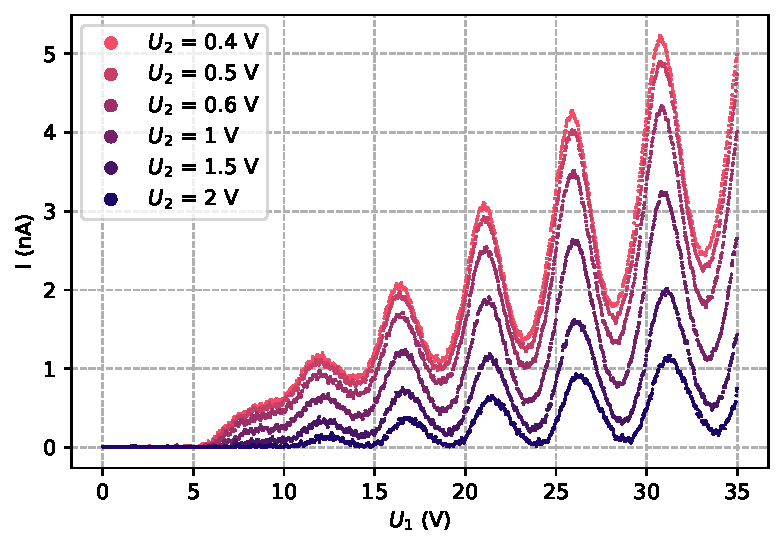
\includegraphics[scale=1.2]{FH_Hg.pdf}
\caption{representación gráfica de los puntos experimentales.}
\label{Fig:1.0}
\end{figure}

\newpage

\begin{figure}[h!]  \centering
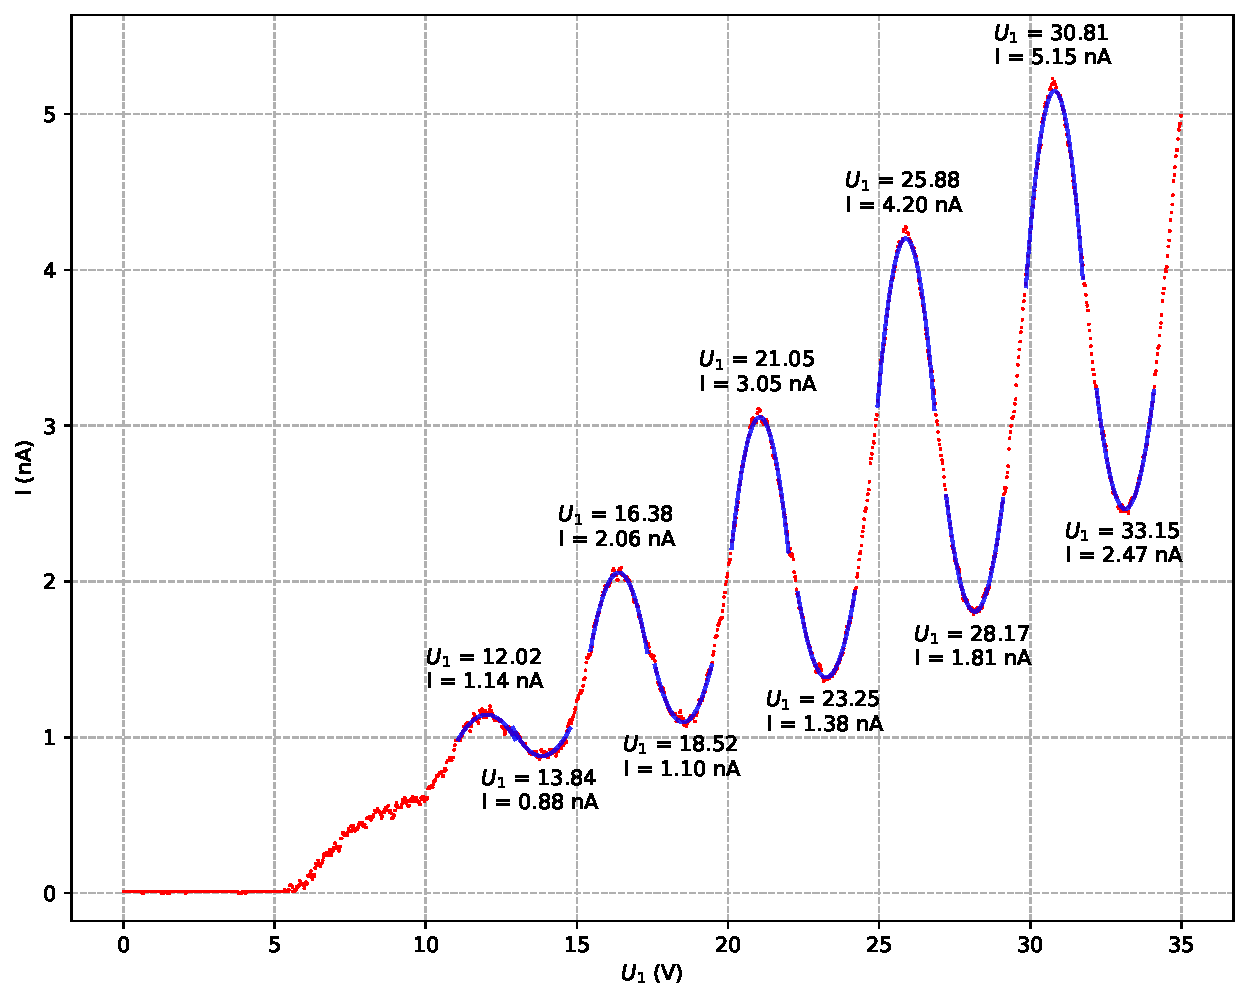
\includegraphics[scale=0.70]{Parabola-1.pdf}
\caption{aproximación parabólica para $U_2=0.4V$.}
\label{Fig:2.1}
\end{figure}


\begin{figure}[h!]  \centering
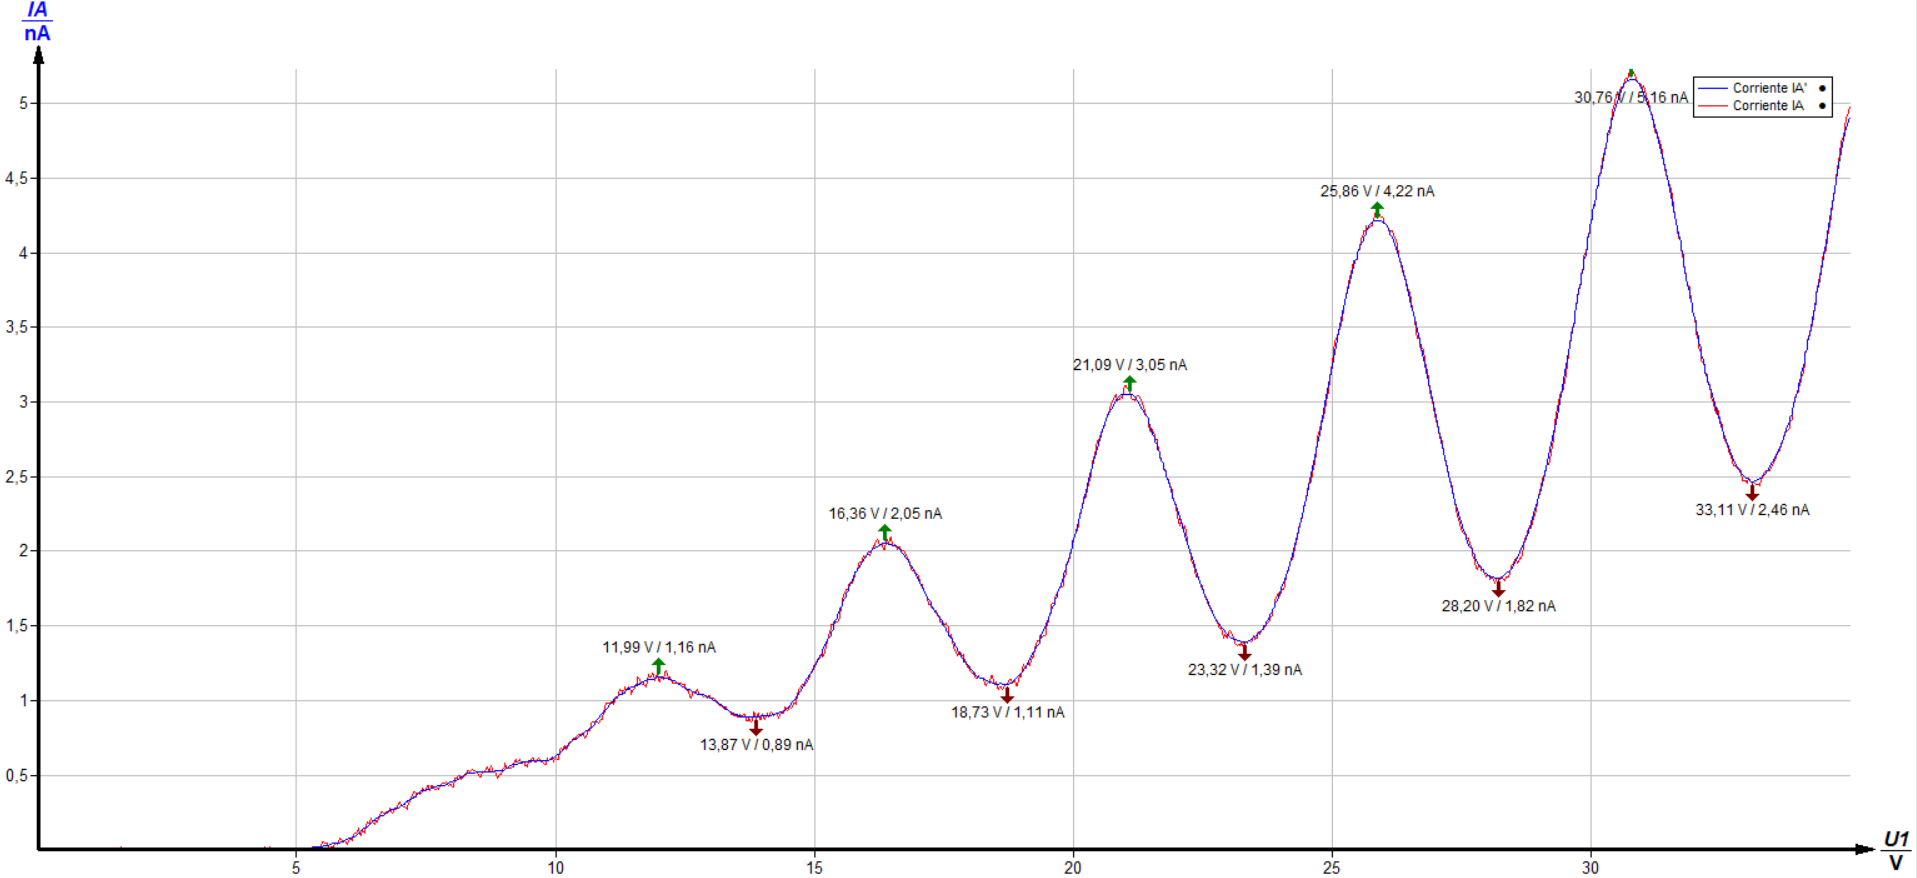
\includegraphics[scale=0.40]{0_4-1.png}
\caption{datos experimentales dados por el programa para $U_2=0.4$V.}
\label{Fig:3.11}
\end{figure}
\newpage
\begin{figure}[h!] \centering
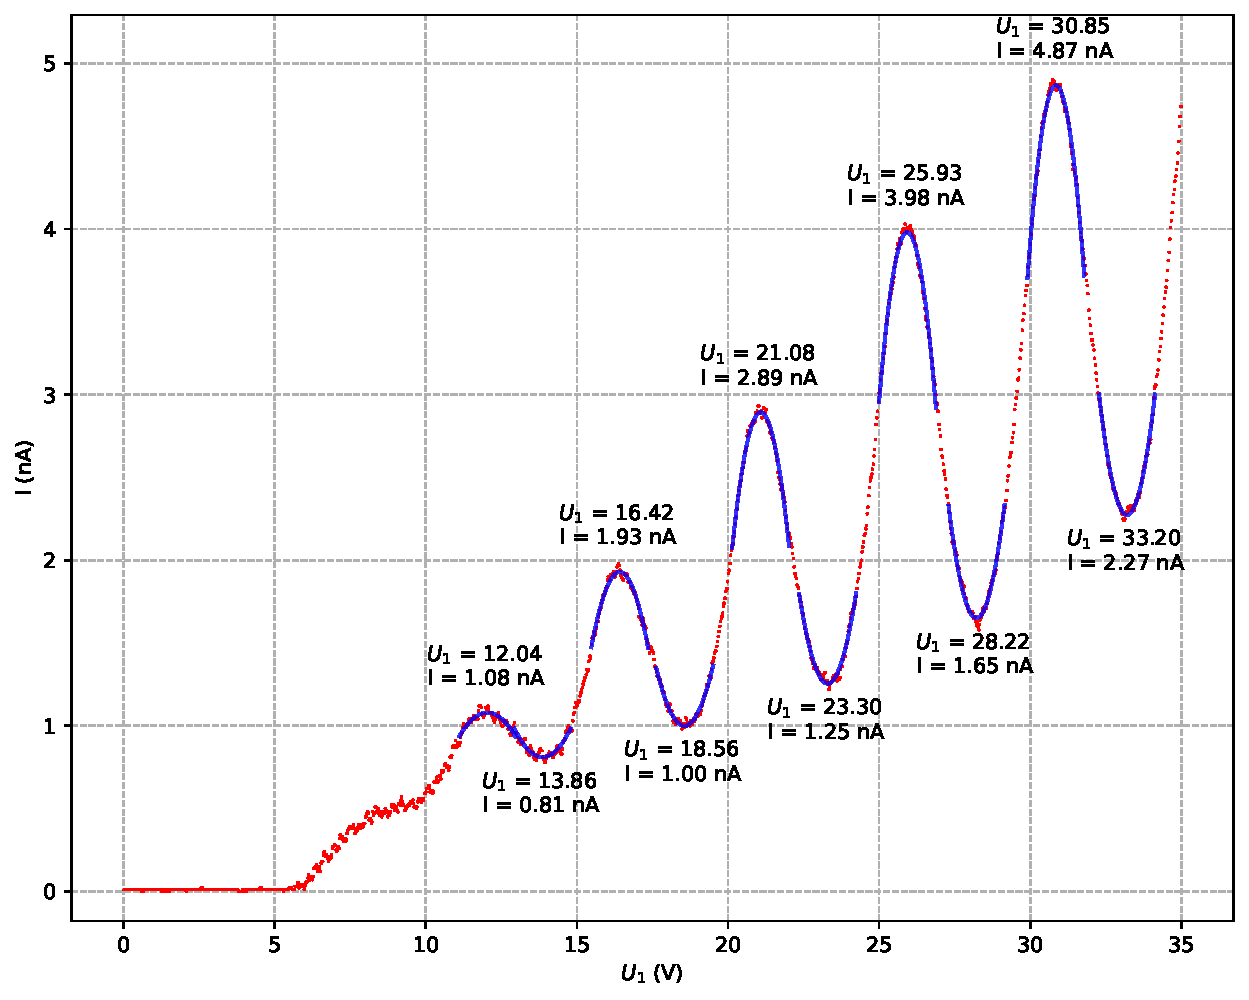
\includegraphics[scale=0.7]{Parabola-2.pdf}
\caption{aproximación parabólica para $U_2=0.5V$.}
\label{Fig:2.2}
\end{figure}

\begin{figure}[h!]  \centering
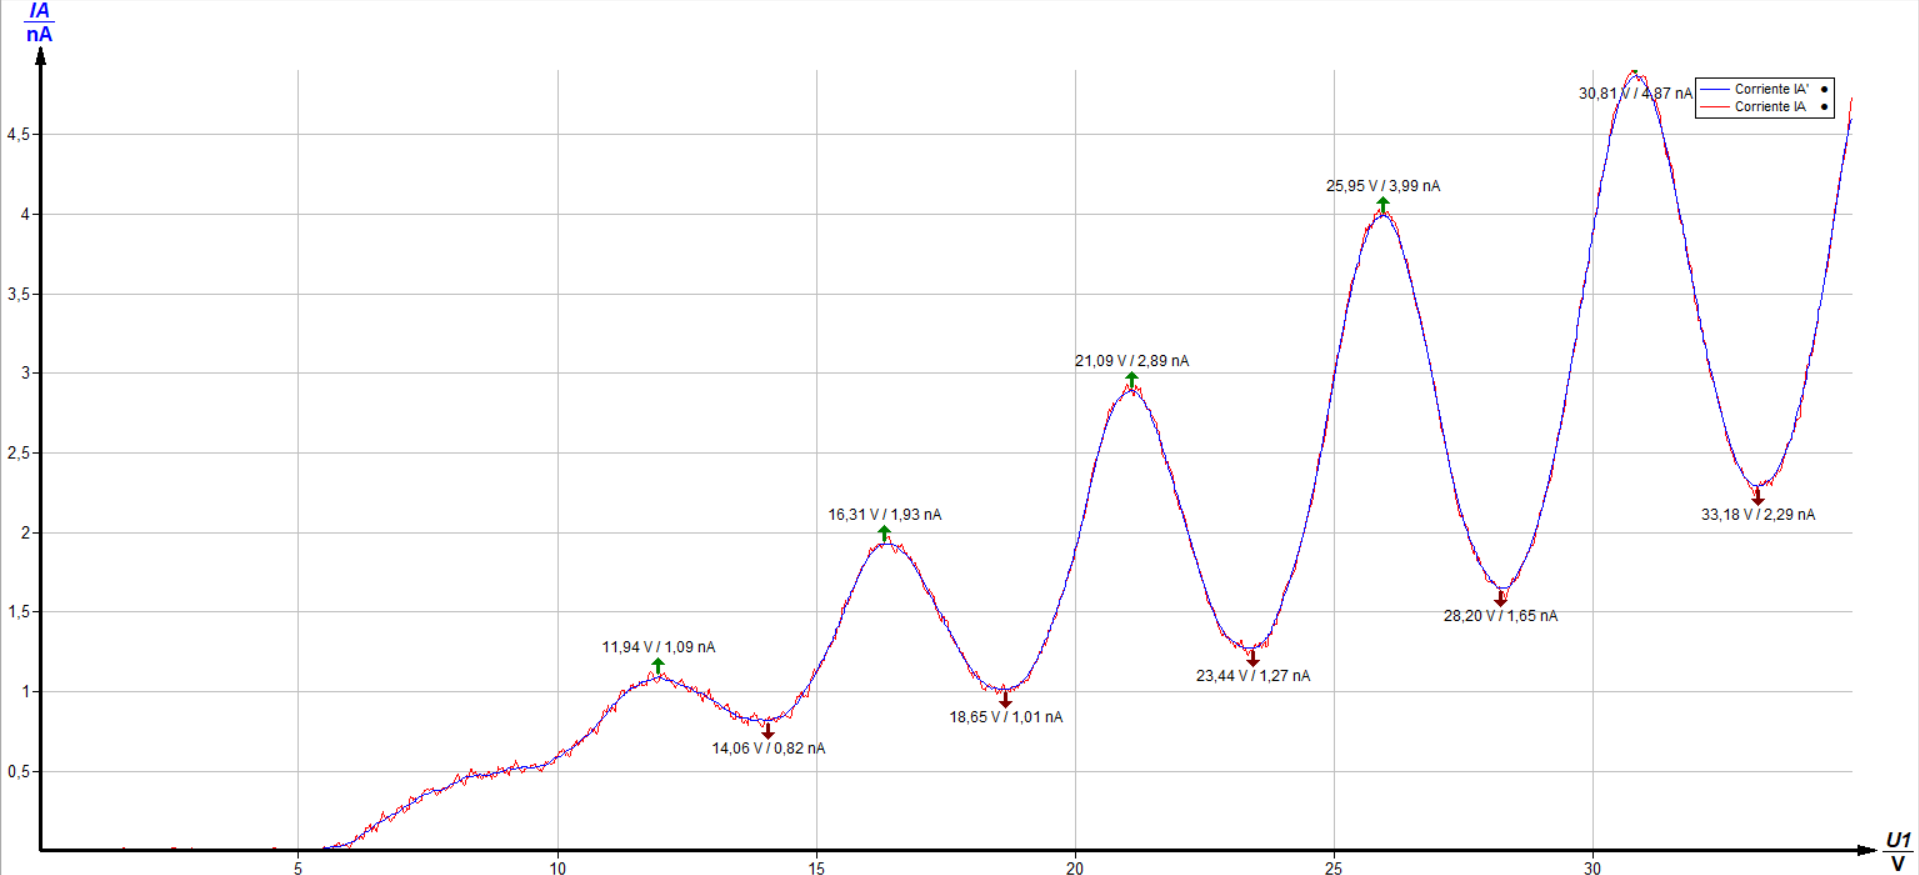
\includegraphics[scale=0.4]{0_5-1.png}
\caption{datos experimentales dados por el programa para $U_2=0.5$V.}
\label{Fig:3.21}
\end{figure}
\newpage
\begin{figure}[h!]  \centering
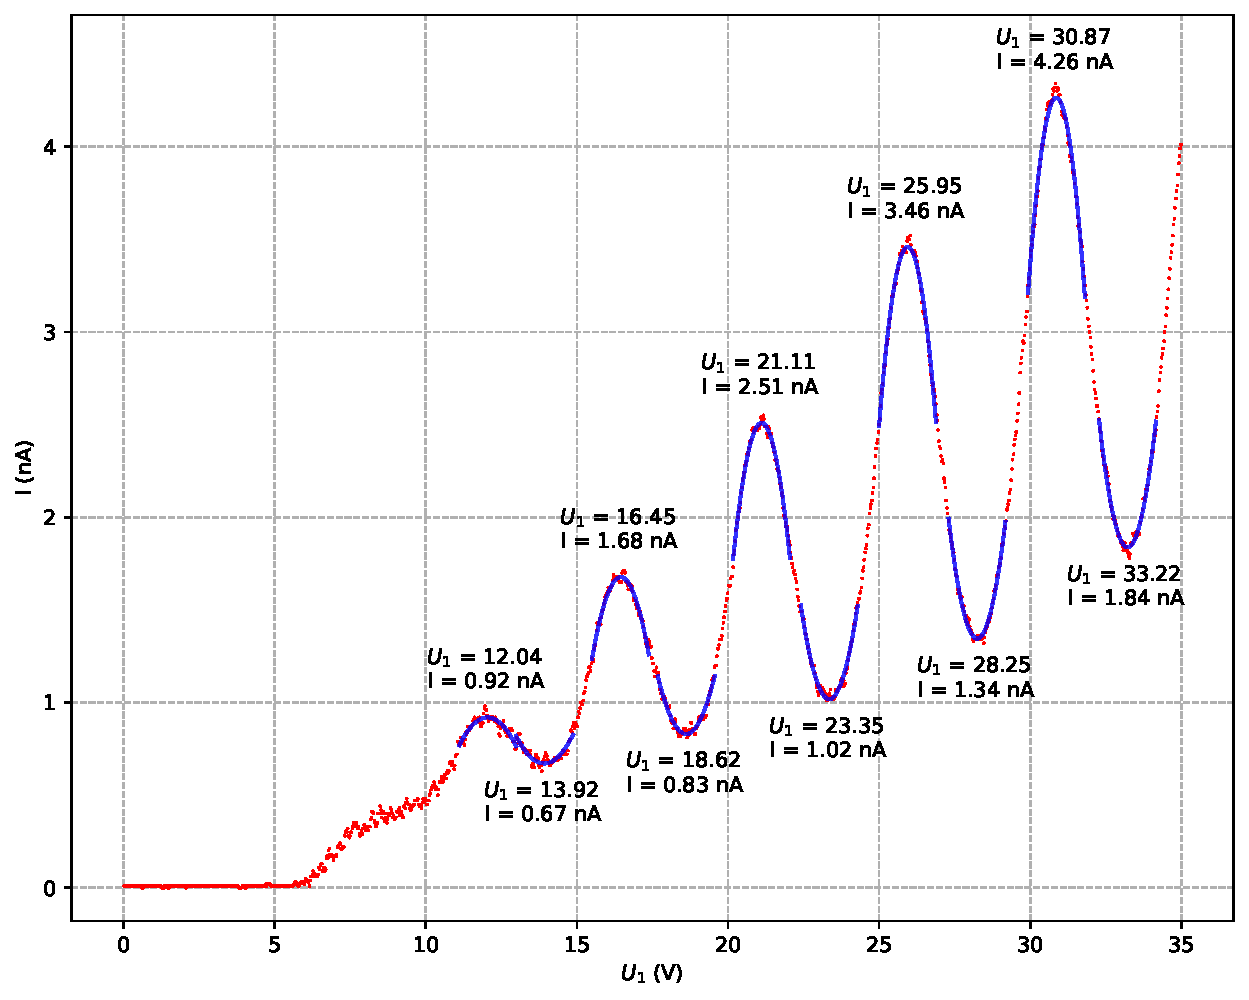
\includegraphics[scale=0.7]{Parabola-3.pdf}
\caption{aproximación parabólica para $U_2=0.6V$.}
\label{Fig:2.3}
\end{figure}

\begin{figure}[h!]  \centering
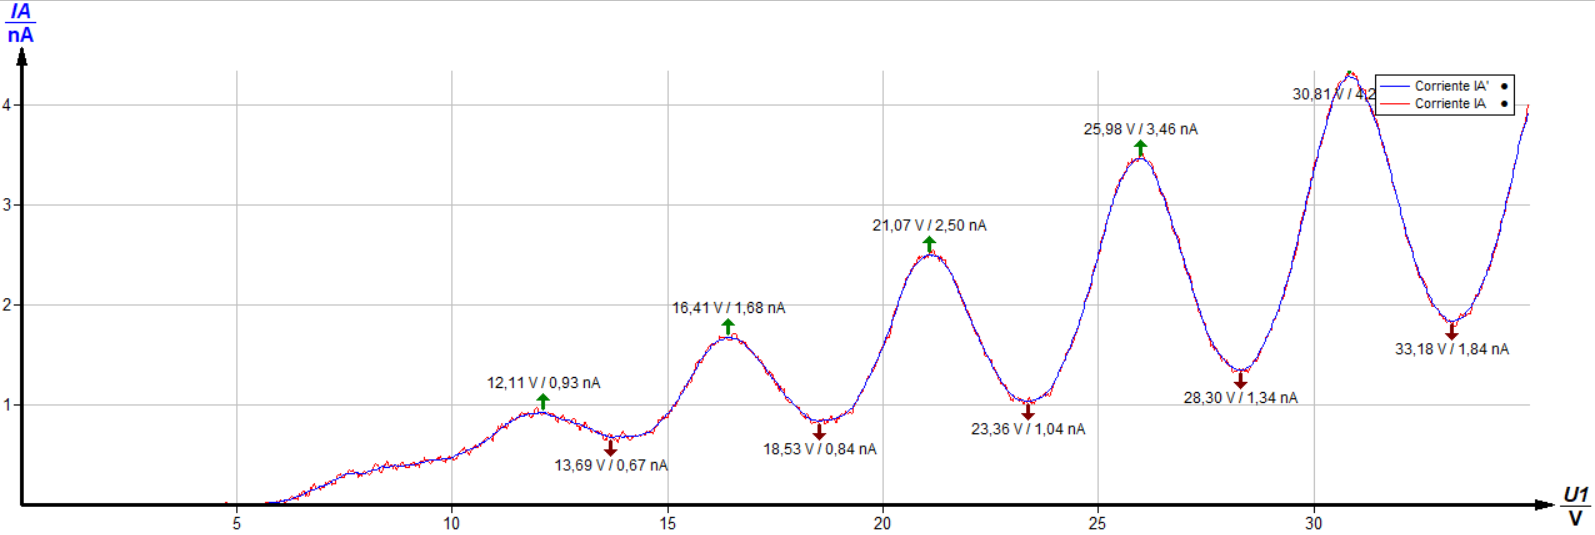
\includegraphics[scale=0.5]{0_6-2.png}
\caption{datos experimentales dados por el programa para $U_2=0.6$V.}
\label{Fig:3.31}
\end{figure}
\newpage
\begin{figure}[h!]  \centering
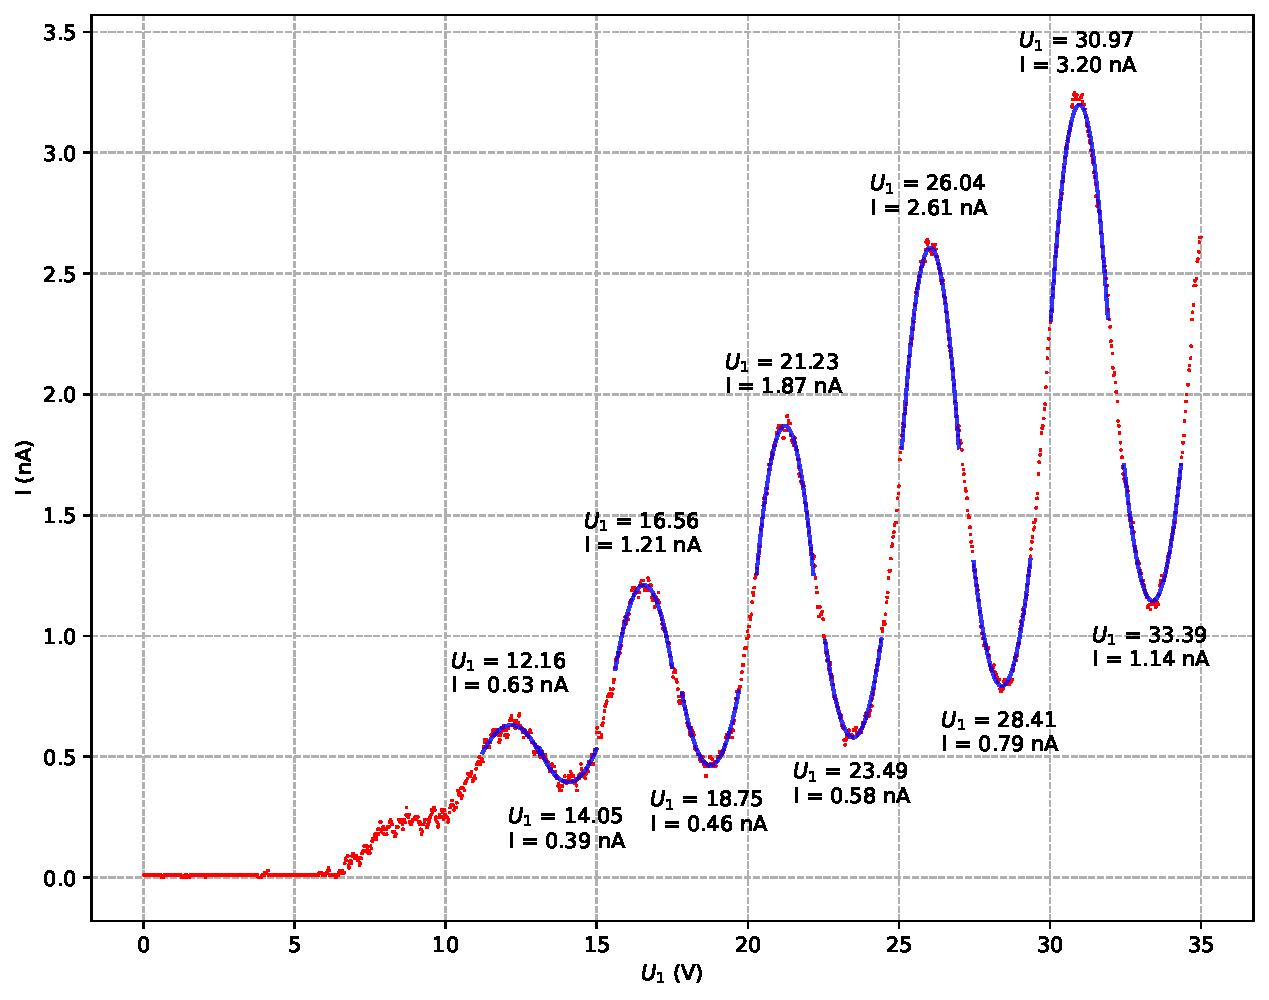
\includegraphics[scale=0.7]{Parabola-4.pdf}
\caption{aproximación parabólica para $U_2=1.0V$.}
\label{Fig:2.4}
\end{figure}

\begin{figure}[h!]  \centering
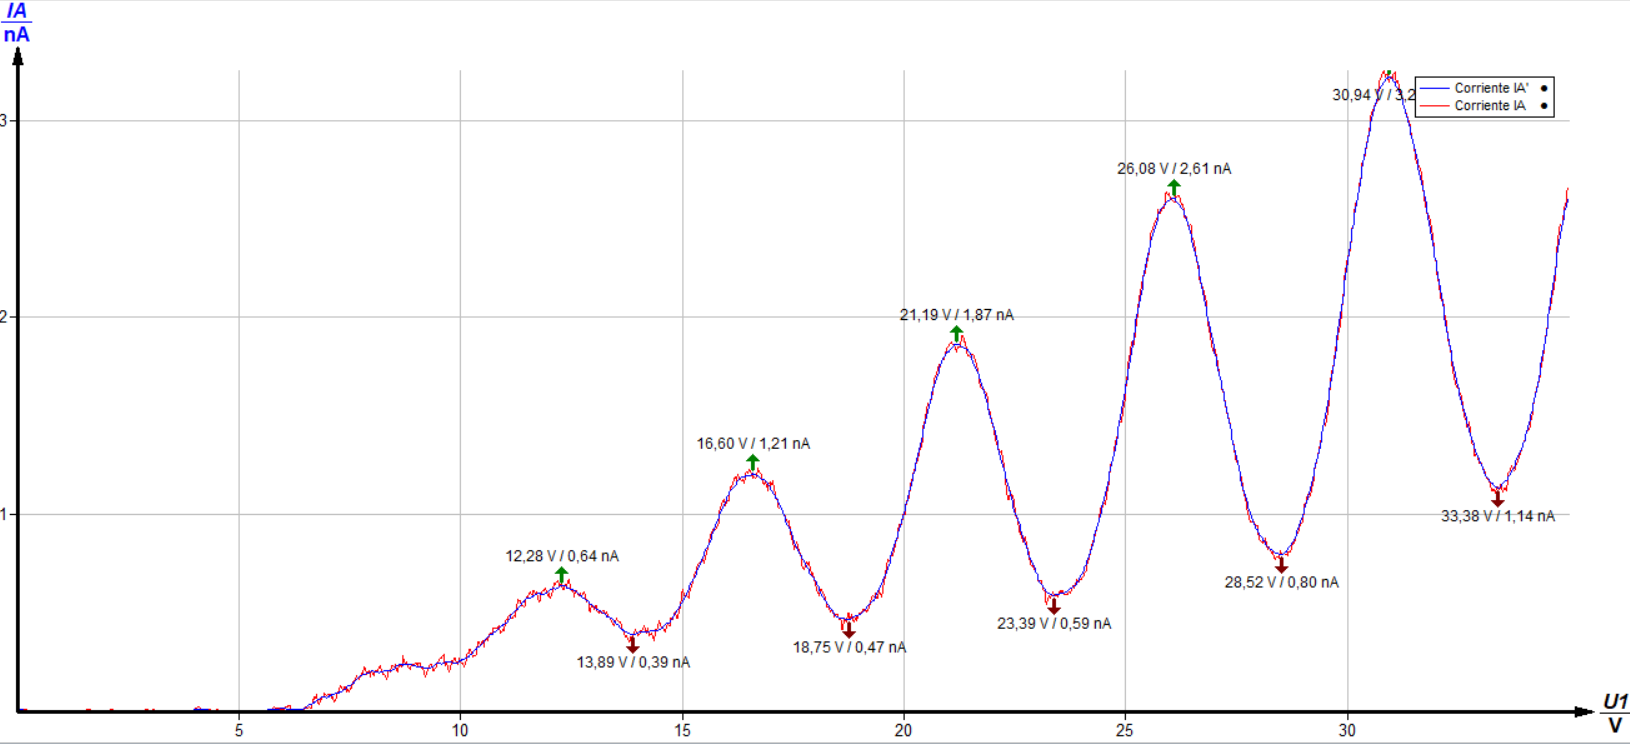
\includegraphics[scale=0.5]{1_0-2.png}
\caption{datos experimentales dados por el programa para $U_2=1.0$V.}
\label{Fig:3.41}
\end{figure}
\newpage
\begin{figure}[h!]  \centering
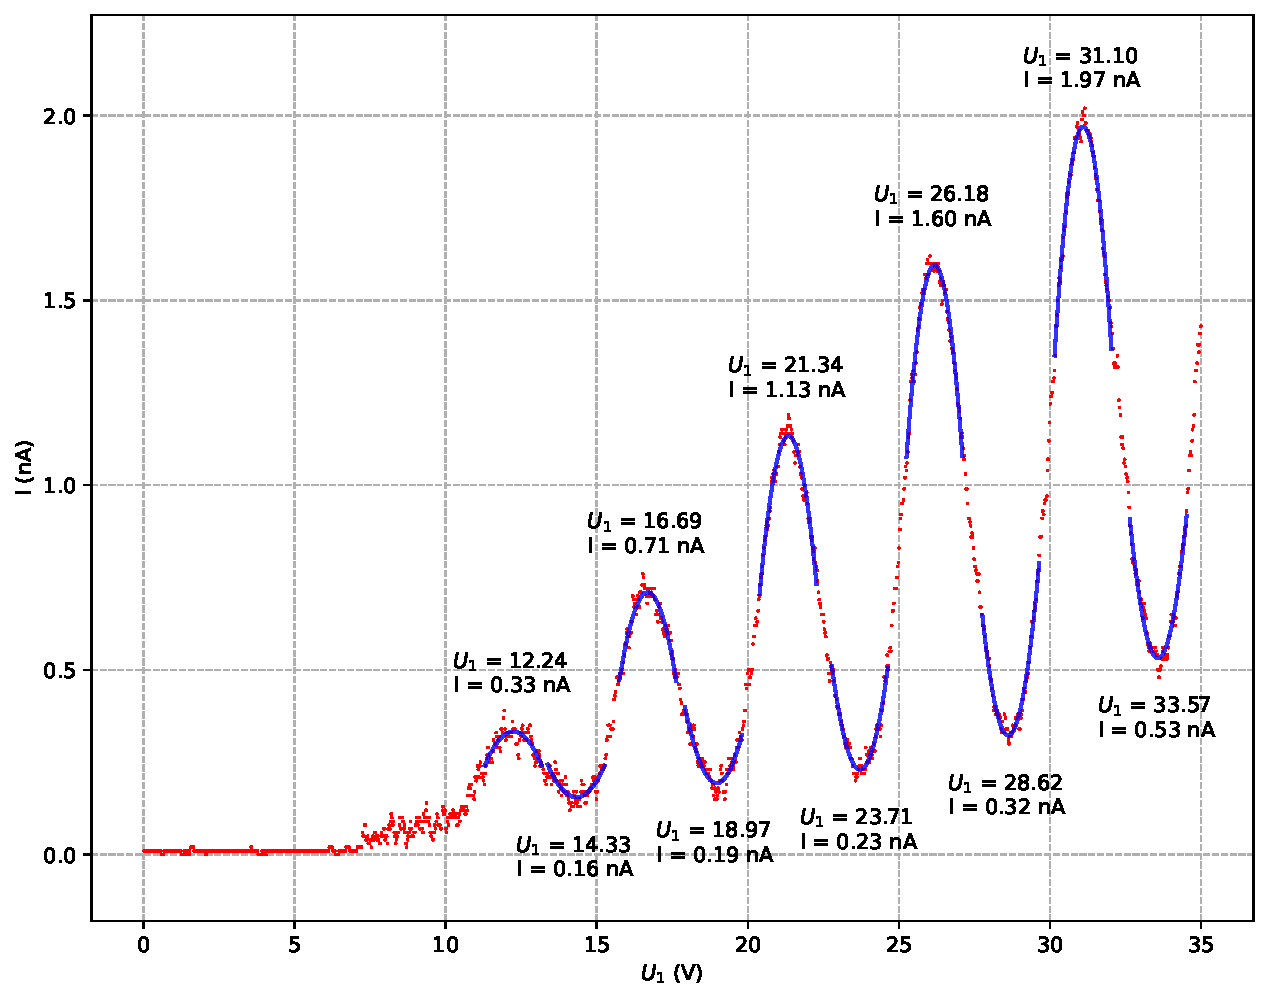
\includegraphics[scale=0.7]{Parabola-5.pdf}
\caption{aproximación parabólica para $U_2=1.5V$.}
\label{Fig:2.5}
\end{figure}

\begin{figure}[h!]  \centering
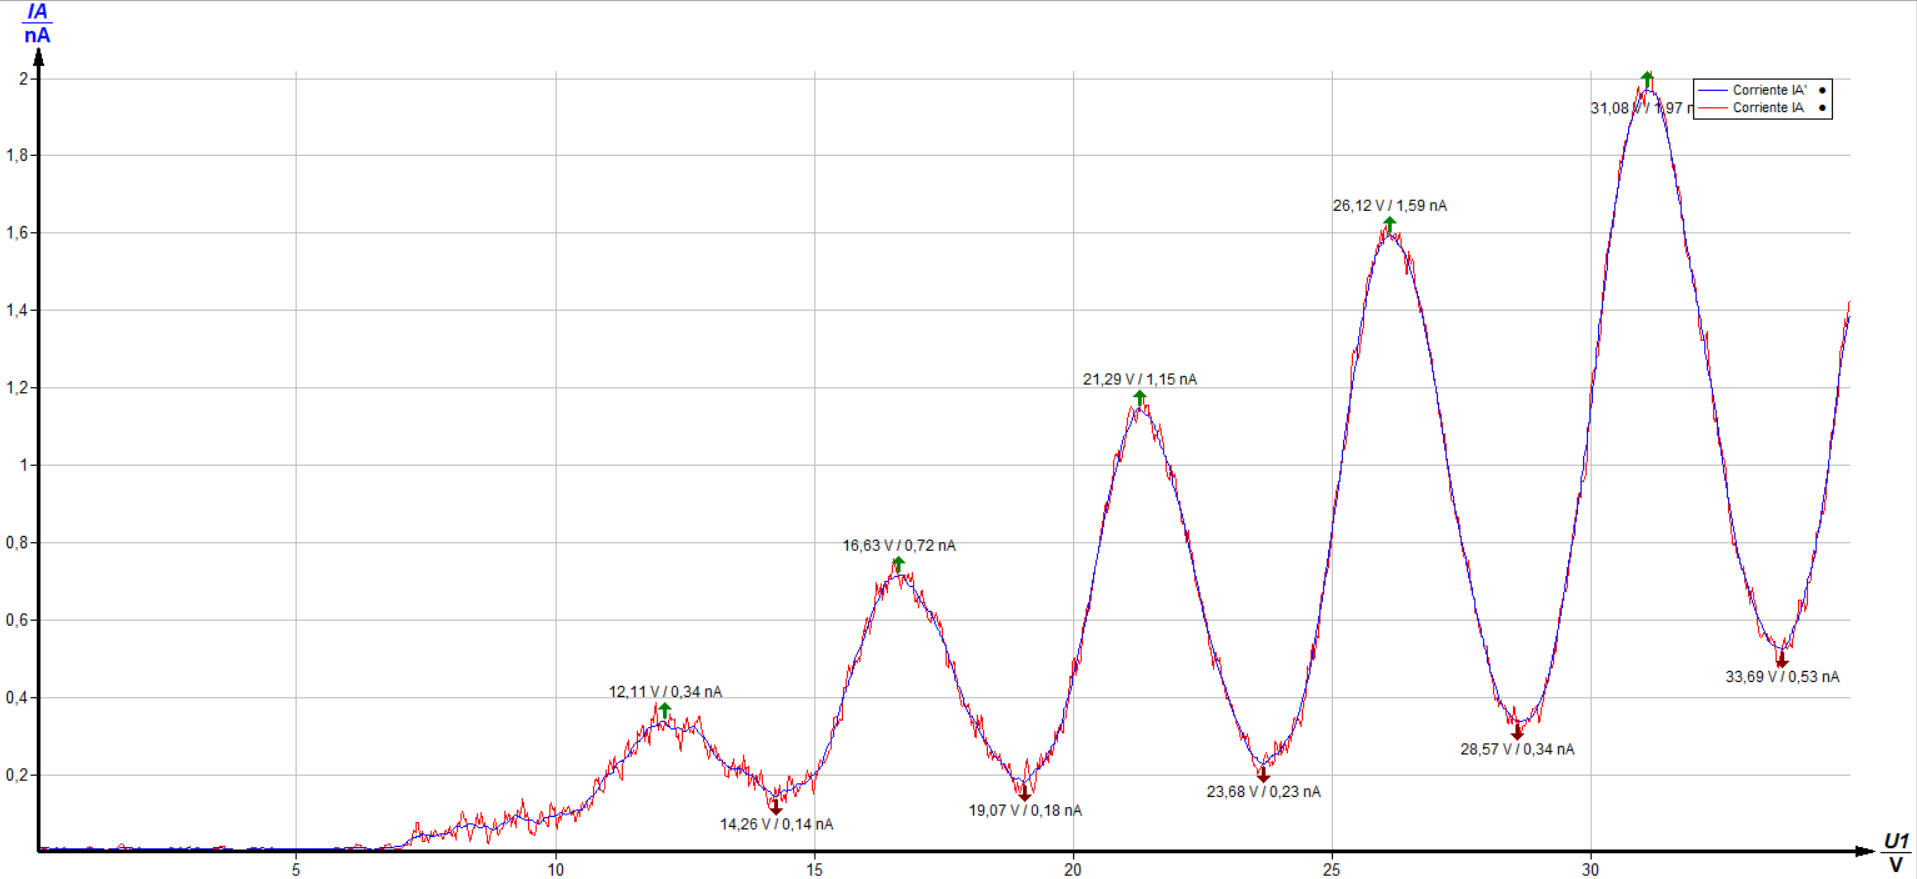
\includegraphics[scale=0.4]{1_5-2.png}
\caption{datos experimentales dados por el programa para $U_2=1.5$V.}
\label{Fig:3.51}
\end{figure}
\newpage
\begin{figure}[h!]  \centering
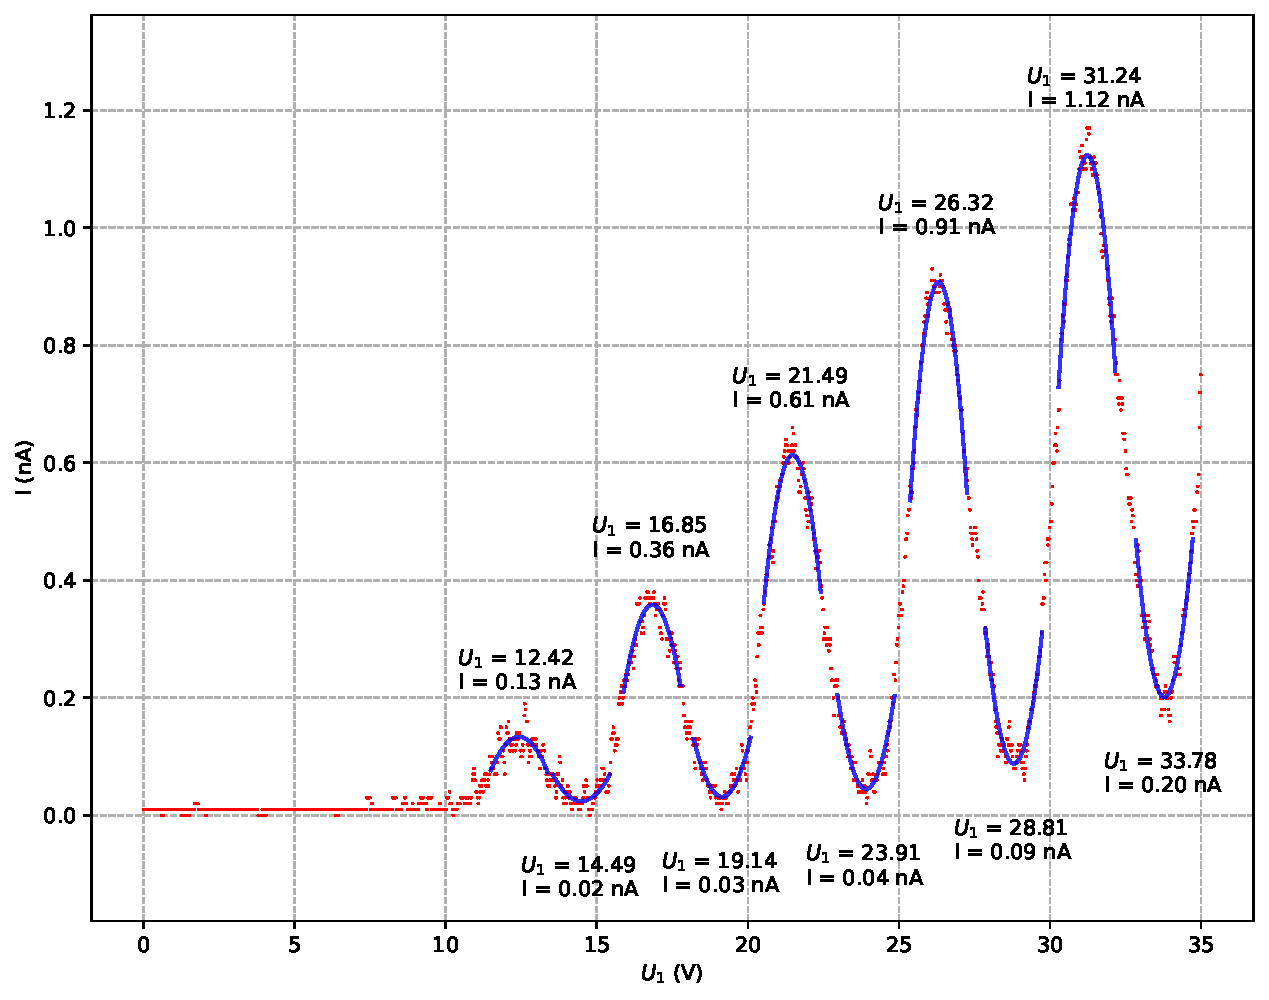
\includegraphics[scale=0.7]{Parabola-6.pdf}
\caption{aproximación parabólica para $U_2=2.0V$.}
\label{Fig:2.6}
\end{figure}

\begin{figure}[h!]  \centering
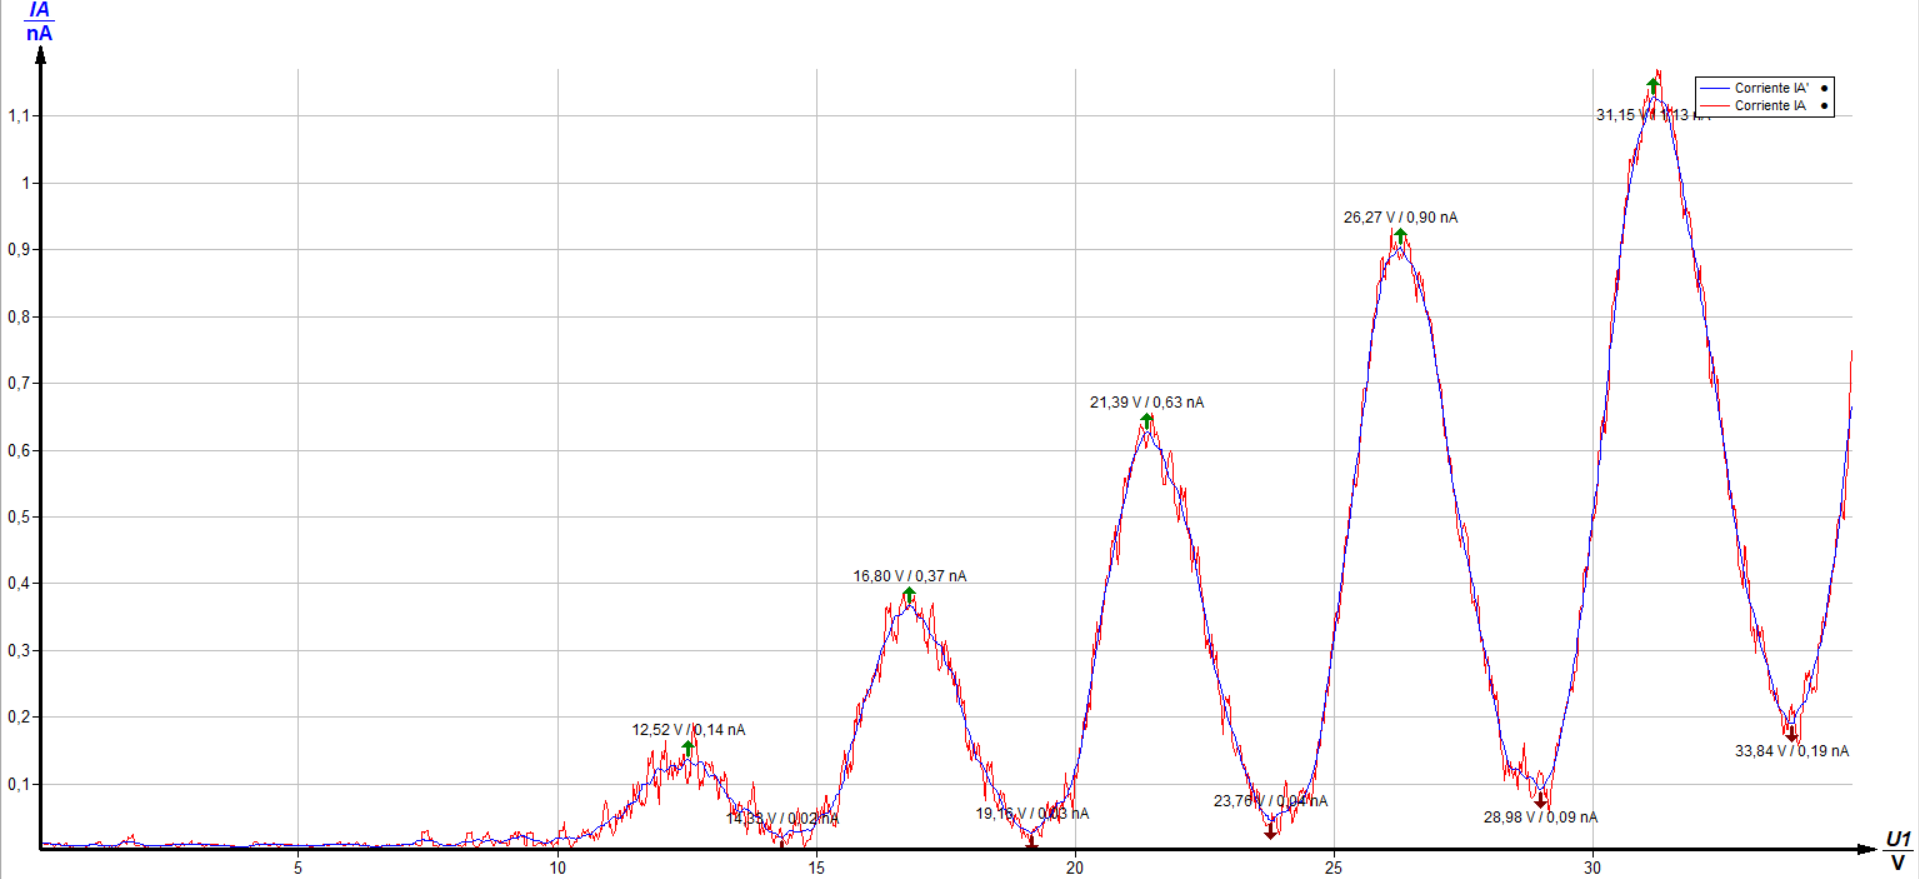
\includegraphics[scale=0.4]{2_0-2.png}
\caption{datos experimentales dados por el programa para $U_2=2.0$V.}
\label{Fig:3.61}
\end{figure}

\newpage

\subsubsection{Representación $\Delta E$ frente al orden del extremo}

\begin{figure}[h!]  \centering
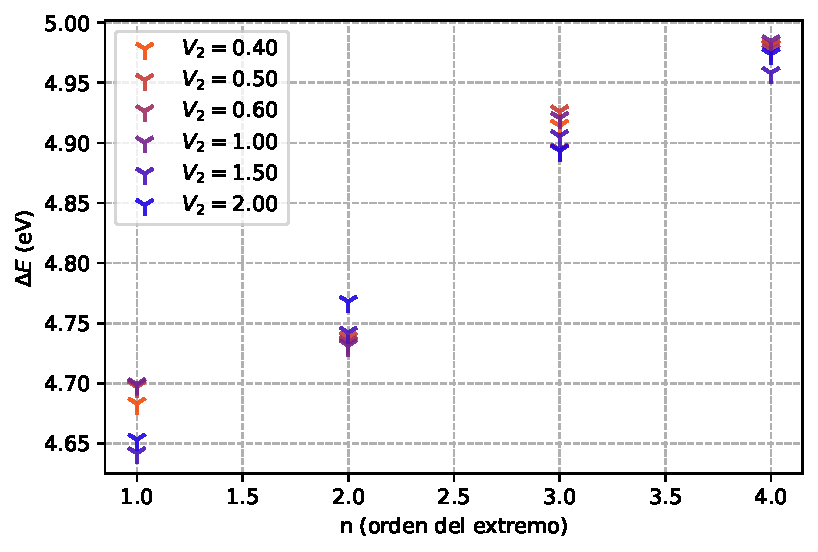
\includegraphics[scale=1.]{Extremo-minimos-par.pdf}
\caption{representación de $\Delta E$ frente al orden del extremo, mínimos parábolas.}
\label{Fig:6.2.2.1}
\end{figure}


\begin{figure}[h!]  \centering
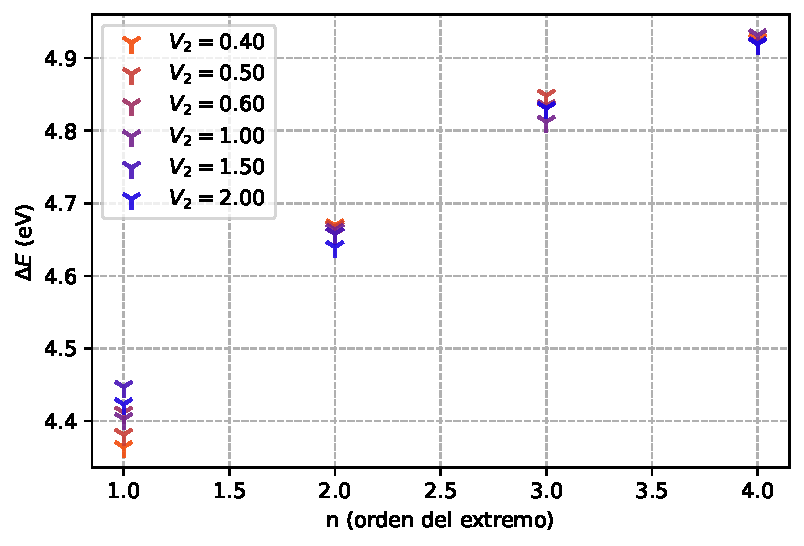
\includegraphics[scale=1.]{Extremo-maximos-par.pdf}
\caption{representación de $\Delta E$ frente al orden del extremo, máximos parábolas.}
\label{Fig:6.2.2.2}
\end{figure}

\newpage

\begin{figure}[h!]  \centering
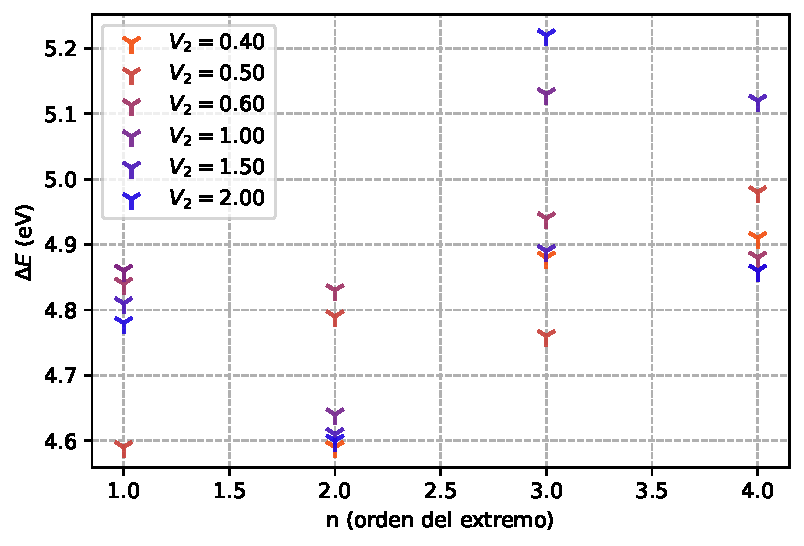
\includegraphics[scale=1.]{Extremo-minimos-lab.pdf}
\caption{representación de $\Delta E$ frente al orden del extremo, mínimos laboratorio.}
\label{Fig:6.2.2.3}
\end{figure}


\begin{figure}[h!]  \centering
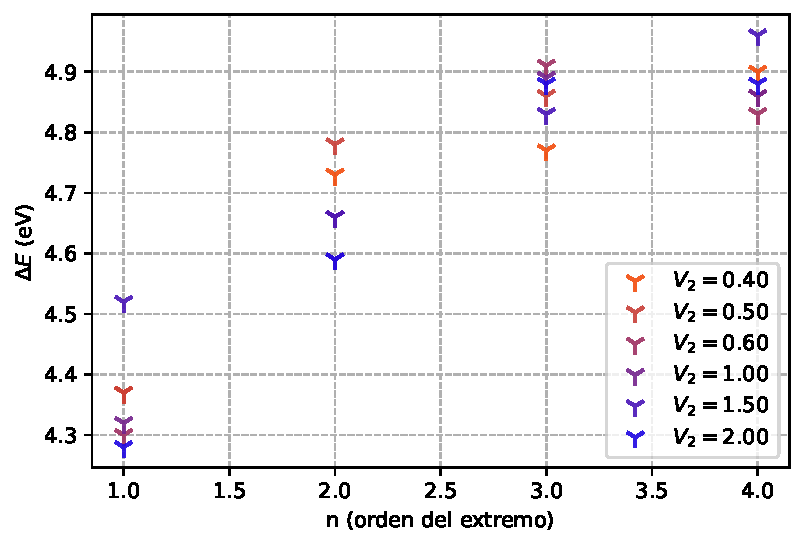
\includegraphics[scale=1.]{Extremo-maximos-lab.pdf}
\caption{representación de $\Delta E$ frente al orden del extremo, máximos laboratorio.}
\label{Fig:6.2.2.4}
\end{figure}

\newpage 


\begin{thebibliography}{n}
\bibitem{libro-1} Luis Miguel Varela Cabo; Faustino Gomez, Jesus Carrete;
{\it Tratamiento de datos físicos}.

\bibitem{paper-1} Varios autores;
{\it Phywe Franck-Hertz experiment with a Hg-tube}.

\bibitem{paper-2} Marnik Metting van Rijn; {\it Franck-Hertz Experiment}
February 8, 2020; ETH-Züric.

\bibitem{paper-2} Varios autores; {\it Guiones Técnicas III Física cuántica}
Universidad de Santiago de Compostela.

\end{thebibliography}



\end{document}